\documentclass[10pt]{article}
\usepackage[letterpaper,margin=1in]{geometry}
\usepackage{times}
\usepackage{microtype}
\usepackage{booktabs}
\usepackage{graphicx}
\usepackage{caption}
\usepackage{float}
\usepackage[section]{placeins}
\usepackage[hidelinks]{hyperref}
\usepackage{amsmath}
\providecommand{\Description}[2][]{}
\captionsetup{font=small,labelfont=bf,skip=6pt}
\captionsetup[table]{position=top,aboveskip=7pt,belowskip=9pt}
\captionsetup[figure]{position=bottom,aboveskip=7pt,belowskip=9pt}
\setlength{\textfloatsep}{20pt plus 3pt minus 2pt}
\setlength{\floatsep}{18pt plus 3pt minus 2pt}
\setlength{\intextsep}{18pt plus 3pt minus 2pt}
\setlength{\tabcolsep}{5pt}
\renewcommand{\arraystretch}{1.08}
\emergencystretch=1em

\title{Selective Query-Side Expansion for Long-Horizon Agent Memory Retrieval}
\author{Salomon DIEI\\School of Computer Science and Engineering, KOREATECH\\\texttt{salomon@koreatech.ac.kr}}
\date{}

\begin{document}
\maketitle

\begin{abstract}
Long-horizon software-engineering agents store prior experience as execution traces,
tool calls, terminal outputs, and error messages, while later retrieval requests are
often phrased as natural-language questions. This representational mismatch can
prevent relevant memories from appearing in the retrieved context. We study
Selective Query-Side Expansion (SQE), a retrieval-time method that expands only
low-confidence queries into hypothetical execution traces and paraphrases, retrieves
each variant against the unchanged memory index, and combines ranked lists with
Reciprocal Rank Fusion. On a 5,000-episode SWE-smith memory store with 500
query-memory pairs, SQE obtains 69.4\% Recall@5,
compared with 69.8\% for dense retrieval and
64.0\% for hybrid RRF. Across 8 independently rebuilt memory-index seeds, SQE averages 69.4\% Recall@5, compared with 68.5\% for dense retrieval, 69.2\% for always-on expansion, and 68.9\% for the executed random-gating budget control. The current evidence supports SQE as a
cost-aware retrieval variant and shows higher Recall@5 than hybrid RRF, but it
does not establish a practically meaningful advantage over dense retrieval or a
clear advantage over the executed random-gating budget control. Downstream Pass@1 evaluation and human-audited query labels remain
necessary before making end-to-end agent-performance claims.
\end{abstract}

\section{Introduction}
Software-engineering agents accumulate long trajectories of observations,
commands, file edits, tests, and error traces. These records are useful only if
future agents can retrieve the relevant fragment when facing a related problem.
The retrieval problem is difficult because the memory and query distributions are
not written in the same style: a stored memory may contain a traceback or a patch
diff, while the future query may ask how an off-by-one line-number bug was fixed.

We study SQE as a retrieval-time intervention. The memory-writing
pipeline remains unchanged. At retrieval time, the method first runs dense
retrieval~\cite{karpukhin2020dpr} and treats the top-1 score as a confidence
signal. If the score is below a threshold, SQE generates execution-style hypothetical traces and paraphrased
queries, retrieves with these variants, and fuses the resulting rankings with
Reciprocal Rank Fusion~\cite{cormack2009rrf}. The method is related to
HyDE~\cite{gao2023hyde}, but is specialized to software-agent traces and is
applied selectively to bound generation cost.

\paragraph{Contributions.}
First, we formulate the trace-query mismatch problem for long-horizon software
agent memory. Second, we implement a selective expansion pipeline that combines
hypothetical traces, paraphrases, dense retrieval, sparse retrieval, and RRF.
Third, we provide a verified retrieval study on SWE-smith trajectories with
8 independently rebuilt memory-index seeds. Fourth, we identify the current
limitations: the confidence gate is weakly calibrated, the evaluation uses
generated retrieval queries, and downstream Pass@1 has not yet been measured.

\section{Related Work}
SQE builds on standard dense and sparse retrieval methods. Dense passage
retrieval maps queries and documents into a shared embedding space, while BM25
uses lexical term matching and remains a useful sparse baseline
~\cite{karpukhin2020dpr,robertson2009bm25}. The SQE experiments keep both
indexes fixed and modify only the query side, so the method can be evaluated as
a retrieval-time intervention rather than a memory-writing change.

Query expansion methods address vocabulary mismatch by rewriting or augmenting
the query before retrieval. HyDE generates a hypothetical document and embeds it
for zero-shot dense retrieval~\cite{gao2023hyde}. SQE uses the same broad idea
of hypothetical query-side expansion, but changes the unit of expansion to
software-agent execution traces and applies expansion only when the initial
retrieval score is low. The generated traces are retrieval probes rather than
claims that those executions actually occurred. Reciprocal Rank Fusion provides
a simple way to combine ranked lists from
the original query, generated traces, paraphrases, and sparse retrieval without
training a ranker~\cite{cormack2009rrf}.

For software-engineering agents, retrieval quality is only an intermediate
signal. SWE-bench-style evaluation measures whether an agent can produce a
patch that resolves a real issue~\cite{jimenez2024swebench}. The present paper
therefore reports retrieval metrics as a controlled diagnostic and treats
Pass@1 task success as required future evidence, not as an implied result.

\section{Method}
Let $M = \{m_i\}_{i=1}^N$ be a memory store of execution traces. Given a
query $q$, dense retrieval returns a ranked list $R_d(q)$ and a top-1 similarity
score $s_1(q)$. SQE expands the query if $s_1(q) < \tau$. For expanded queries,
an LLM generates $K$ hypothetical traces and $P$ paraphrases. Each variant is
retrieved against the same dense and BM25 sparse indexes~\cite{robertson2009bm25}. The ranked lists are fused
using RRF:
\[
  \mathrm{score}(m) = \sum_j \frac{1}{k + \mathrm{rank}_j(m)}.
\]
The current implementation uses $\tau=0.65$, $K=2$, $P=2$, and $k=60$.

Figure~\ref{fig:method-overview} shows the retrieval path. The high-confidence
branch uses the initial dense list. The low-confidence branch generates trace
probes and paraphrases, retrieves each query variant, and sends all ranked lists
to RRF.

\begin{figure}[!tbp]
\centering
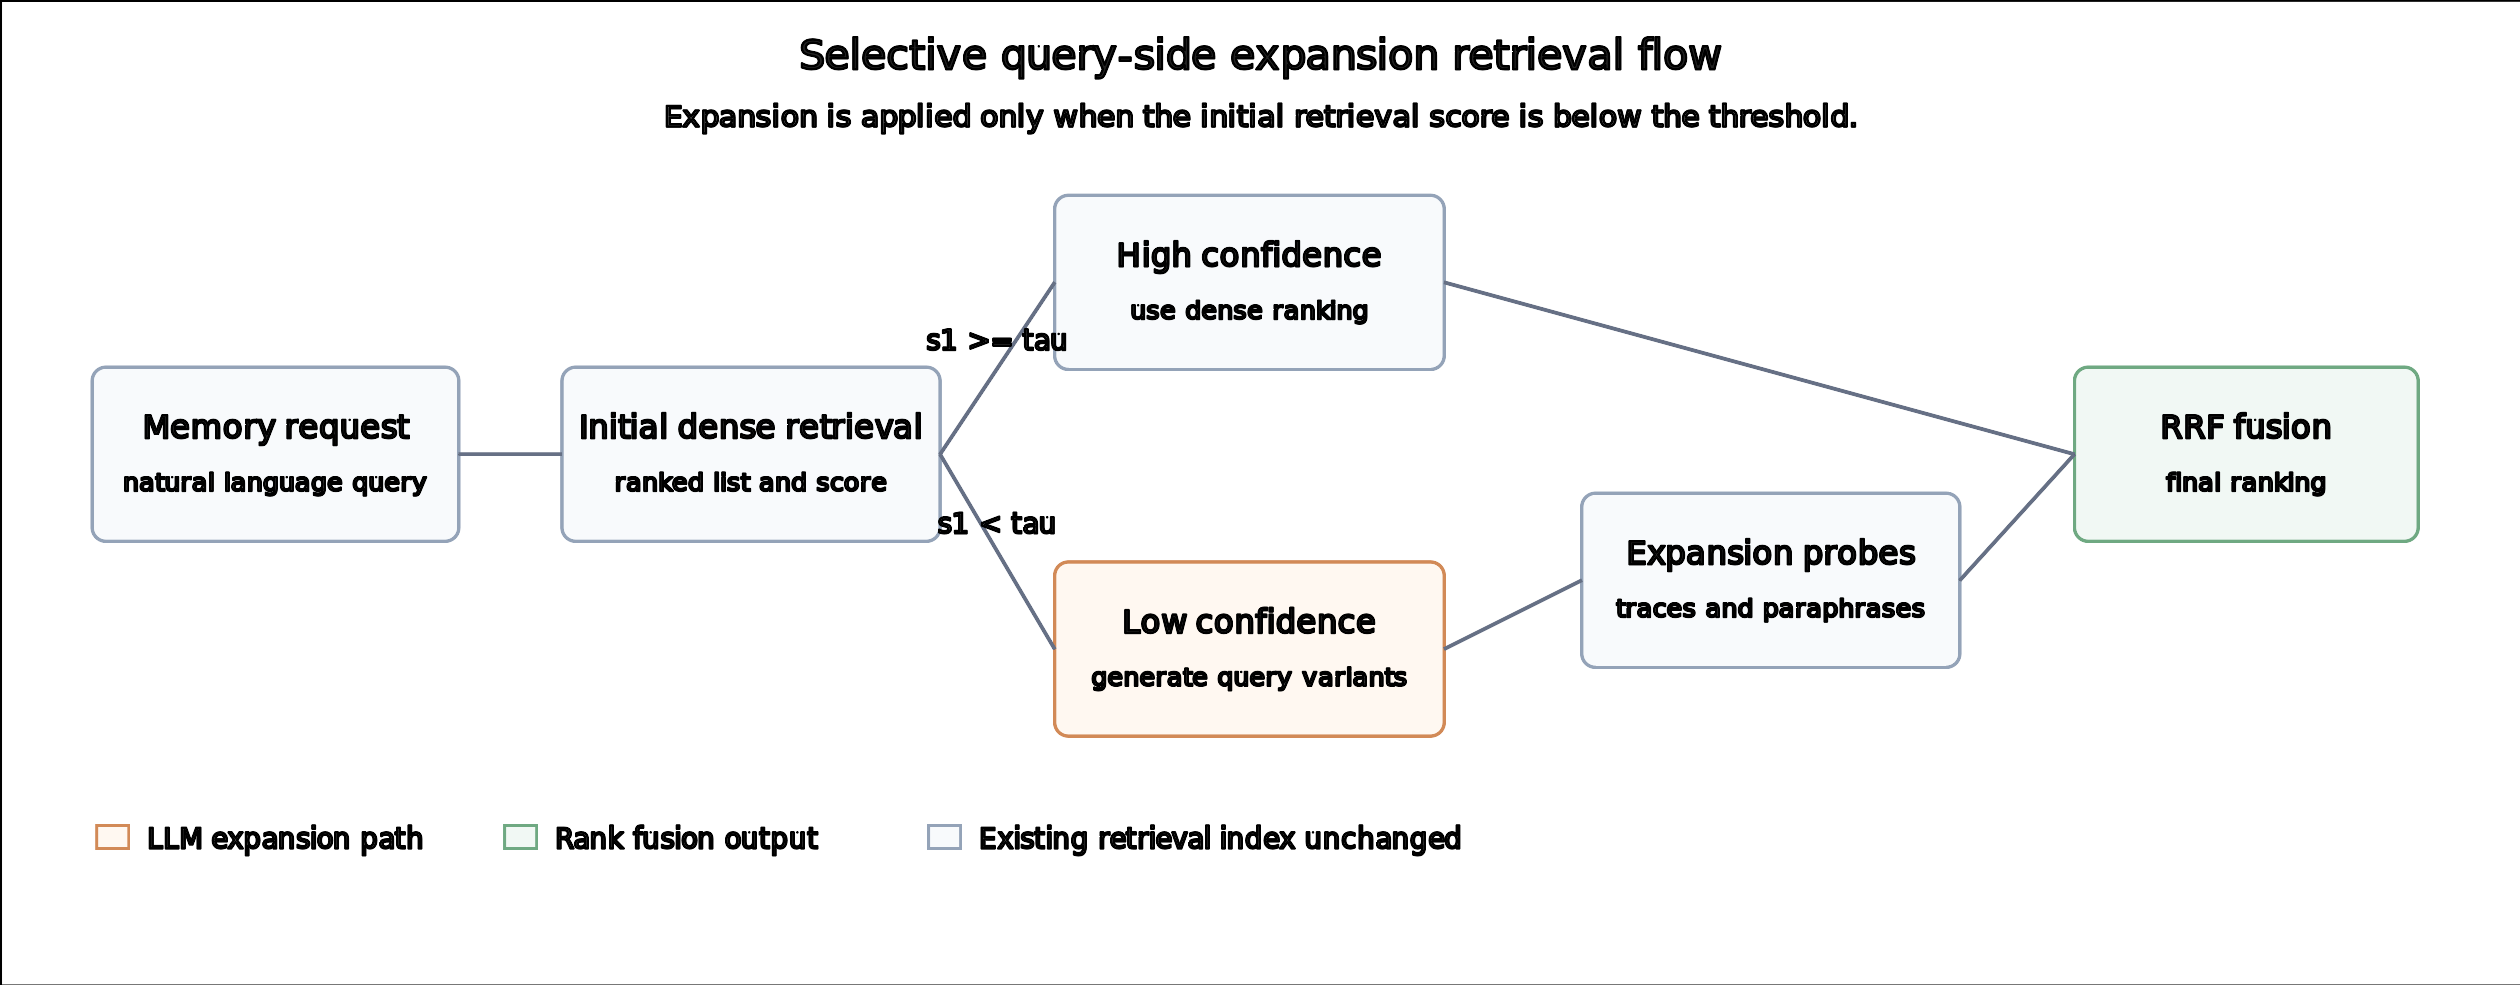
\includegraphics[width=0.92\linewidth]{figures/method_overview.png}
\caption{SQE retrieval flow. The method changes only the query side at retrieval time; the memory store and index are left unchanged.}
\Description{Flow diagram showing dense retrieval, a confidence gate, query-side trace and paraphrase expansion for low-confidence queries, parallel retrieval, and Reciprocal Rank Fusion.}
\label{fig:method-overview}
\end{figure}

\section{Experimental Setup}
\begin{table}[!tbp]
\caption{Experiment configuration and release placeholders.}
\label{tab:setup}
\centering
\small
\begin{tabular}{ll}
\toprule
Item & Value \\
\midrule
Memory episodes & -- \\
Evaluation queries & 500 \\
Dataset split & -- \\
Evaluation source & -- \\
Dataset seed & -- \\
Embedding model & BAAI/bge-m3 \\
Generator model & Qwen3.6-35B-A3B via vLLM \\
Index & FAISS dense + BM25 sparse \\
Fusion & Reciprocal Rank Fusion \\
GitHub URL & \href{https://github.com/Salomondiei08/sqe-experiment}{source repository} \\
Hugging Face dataset & \href{https://huggingface.co/datasets/TheReinventGuy/sqe-experiment}{released artifacts} \\
\bottomrule
\end{tabular}

\end{table}

Table~\ref{tab:setup} summarizes the current retrieval benchmark. The
experiment uses generated natural-language queries paired with
target memories. This setup isolates retrieval, but it does not yet establish
downstream task success. A complete evaluation requires verified human-audit
labels and agent Pass@1 evaluation on SWE-bench-style tasks~\cite{jimenez2024swebench}.
Random-Gated-Expansion is an executed control: it runs the same
expansion-and-retrieval code as SQE, but replaces the confidence gate with seeded
random expansion decisions at a comparable expansion rate and stores the
resulting per-query rows in JSONL.

\section{Results}
We treat the 8-seed aggregate in Table~\ref{tab:multiseed} as the primary
retrieval evidence. Table~\ref{tab:seed42} is retained as a detailed audit
anchor because its per-query rows, cost traces, figures, and case analyses are
all regenerated by the artifact pipeline.

\begin{table}[!tbp]
\caption{Seed-42 retrieval results used as the detailed audit anchor.}
\label{tab:seed42}
\centering
\small
\begin{tabular}{lrrrrr}
\toprule
Method & Recall@1 & Recall@5 & Recall@10 & MRR & Expansion \%
\\
\midrule
Dense-Only & 49.0 & 69.8 & 75.4 & 57.4 & -- \\
BM25-Only & 17.6 & 31.4 & 35.8 & 23.3 & -- \\
Hybrid-RRF & 35.4 & 64.0 & 73.2 & 47.4 & -- \\
Paraphrases-Only & 47.0 & 68.2 & 75.0 & 56.0 & 100.0 \\
HyDE-Traces-Only & 36.2 & 64.0 & 70.4 & 47.9 & 100.0 \\
Always-Expand & 42.2 & 68.0 & 75.6 & 53.2 & 100.0 \\
Random-Gated-Expansion & 46.0 & 69.0 & 75.8 & 55.3 & 47.0 \\
Selective-QE & 47.2 & 69.4 & 75.4 & 56.4 & 46.0 \\
\bottomrule
\end{tabular}

\end{table}

In the seed-42 run, SQE changes Recall@5 by -0.4 percentage points relative to dense-only
retrieval and +5.4 percentage points relative to hybrid RRF
in the current run. Recall@1 is lower than dense retrieval. This indicates that
the current SQE configuration has higher Recall@5 than hybrid RRF,
but does not improve the strongest dense baseline. The always-on ablation shows
that expanding every query can hurt Recall@1, so selectivity is mainly a
cost-control mechanism in this run.

\subsection{Multi-seed retrieval aggregate}
\begin{table}[!tbp]
\caption{Aggregate retrieval results over independent memory-index seeds.}
\label{tab:multiseed}
\centering
\small
\begin{tabular}{lrrrr}
\toprule
Method & Seeds & Recall@1 & Recall@5 & Recall@10 \\
\midrule
Dense-Only & 8 & 45.5 $\pm$ 3.1 & 68.5 $\pm$ 2.7 & 74.2 $\pm$ 2.5 \\
Hybrid-RRF & 8 & 32.5 $\pm$ 1.5 & 63.5 $\pm$ 2.5 & 71.8 $\pm$ 2.6 \\
Always-Expand & 8 & 39.8 $\pm$ 3.1 & 69.2 $\pm$ 3.4 & 75.9 $\pm$ 2.3 \\
Random-Gated-Expansion & 8 & 42.6 $\pm$ 2.9 & 68.9 $\pm$ 3.0 & 75.0 $\pm$ 2.6 \\
Selective-QE & 8 & 44.5 $\pm$ 3.4 & 69.4 $\pm$ 2.7 & 75.3 $\pm$ 2.2 \\
\bottomrule
\end{tabular}

\end{table}

The aggregate uses 8 independently sampled memory stores of 5,000 episodes each and rebuilt
indices. SQE has slightly higher mean Recall@5 than dense retrieval, but the
paired effect against dense retrieval is small and Recall@1 remains below dense
retrieval. The result is therefore evidence for a modest retrieval-only
candidate-set difference under this setup, not strong evidence of an end-to-end
agent improvement. Figure~\ref{fig:recall} reports the
seed-42 method comparison, while Table~\ref{tab:paired-multiseed} reports the
paired aggregate uncertainty.

\begin{table}[!tbp]
\caption{Paired bootstrap tests over all independent memory-index seeds.}
\label{tab:paired-multiseed}
\centering
\scriptsize
\begin{tabular}{lrrrr}
\toprule
Baseline & Queries & $\Delta$R@5 & 95\% CI & Bootstrap $p$ \\
\midrule
Dense-Only & 4000 & +0.9 & [+0.1, +1.7] & 0.015 \\
Hybrid-RRF & 4000 & +5.9 & [+4.8, +7.0] & 0.000 \\
Always-Expand & 4000 & +0.1 & [-0.4, +0.7] & 0.315 \\
Random-Gated-Expansion & 4000 & +0.5 & [-0.2, +1.1] & 0.085 \\
Paraphrases-Only & 4000 & +1.1 & [+0.3, +1.9] & 0.005 \\
HyDE-Traces-Only & 4000 & +5.6 & [+4.7, +6.6] & 0.000 \\
\bottomrule
\end{tabular}

\end{table}

The paired bootstrap over all 4,000 query rows estimates a
small Recall@5 improvement over dense retrieval: the Recall@5 difference against dense retrieval is 0.9 points with a 95\% interval of [0.1, 1.7]. The
same test shows larger gains over hybrid RRF and trace-only expansion, but not
a clear advantage over the executed random-gating budget control.
At the query level, SQE recovers 140 top-5 targets missed by Dense-Only, but loses 105 targets that Dense-Only retrieved, for a net change of 35 over 4,000 paired queries. Table~\ref{tab:win-loss} reports the corresponding
win/loss counts.

\begin{table}[!tbp]
\caption{Query-level top-5 wins and losses for SQE against Dense-Only.}
\label{tab:win-loss}
\centering
\small
\begin{tabular}{lrrrrrr}
\toprule
Split & N & Both hit & SQE win & SQE loss & Both miss & Net \\
\midrule
seed 42 & 500 & 334 & 13 & 15 & 138 & -2 \\
seed 43 & 500 & 314 & 18 & 18 & 150 & 0 \\
seed 44 & 500 & 347 & 17 & 13 & 123 & 4 \\
seed 45 & 500 & 335 & 18 & 10 & 137 & 8 \\
seed 46 & 500 & 350 & 16 & 11 & 123 & 5 \\
seed 47 & 500 & 320 & 17 & 15 & 148 & 2 \\
seed 48 & 500 & 322 & 22 & 11 & 145 & 11 \\
seed 49 & 500 & 313 & 19 & 12 & 156 & 7 \\
\midrule
All & 4000 & 2635 & 140 & 105 & 1120 & 35 \\
\bottomrule
\end{tabular}

\end{table}

Table~\ref{tab:cases} lists deterministic examples from the seed-42 retrieval
rows. They are illustrative only and are not additional aggregate metrics.

\begin{table}[!tbp]
\caption{Seed-42 examples where SQE and Dense-Only differ at top-5.}
\label{tab:cases}
\centering
\scriptsize
\resizebox{\linewidth}{!}{\begin{tabular}{lllllp{0.45\linewidth}}
\toprule
Case & Query ID & Dense rank & SQE rank & Expanded & Query \\
\midrule
SQE gain & q\_0014 & >10 & 3 & yes & What regular expression pattern was used to define the digit group variable? \\
SQE gain & q\_0063 & 8 & 3 & yes & Did the test script confirm that the parser correctly handles NULL comparisons... \\
SQE loss & q\_0002 & 1 & 7 & yes & Did the test script confirm that the fix for the FOO value was successful? \\
SQE loss & q\_0031 & 1 & 7 & yes & What was the output when I ran the simple test script to verify the initial cal... \\
\bottomrule
\end{tabular}
}
\end{table}

\subsection{Expansion cost}
\begin{table}[!tbp]
\caption{Estimated expansion cost for each retrieval method.}
\label{tab:cost}
\centering
\small
\begin{tabular}{lrr}
\toprule
Method & Expansion \% & Estimated LLM calls/query \\
\midrule
Dense-Only & -- & 0.00 \\
BM25-Only & -- & 0.00 \\
Hybrid-RRF & -- & 0.00 \\
Paraphrases-Only & 100.0 & 1.00 \\
HyDE-Traces-Only & 100.0 & 2.00 \\
Always-Expand & 100.0 & 3.00 \\
Random-Gated-Expansion & 47.0 & 1.41 \\
Selective-QE & 46.0 & 1.38 \\
\bottomrule
\end{tabular}

\end{table}

The completed ablations estimate generation cost by counting LLM calls rather
than provider-reported tokens. Selective-QE uses fewer expansion calls than
always-on expansion because it expands 46.0\% of queries.
The measured-token reruns below provide provider-reported token usage for all expansion ablations. Table~\ref{tab:cost} reports estimated calls, and
Table~\ref{tab:tokens} reports the measured-token reruns.

\subsection{Measured token cost}
\begin{table}[!tbp]
\caption{Provider-reported token usage for measured-token reruns.}
\label{tab:tokens}
\centering
\scriptsize
\begin{tabular}{lrrrrr}
\toprule
Method & Expanded & Calls/q & Prompt tok/q & Total tok/q & Latency s/q \\
\midrule
Selective-QE & 46.0 & 1.38 & 209.2 & 405.1 & 2.77 \\
Always-Expand & 100.0 & 2.99 & 455.5 & 899.3 & 5.37 \\
HyDE-Traces-Only & 100.0 & 2.00 & 367.0 & 758.2 & 3.99 \\
Paraphrases-Only & 100.0 & 1.00 & 88.5 & 131.6 & 1.02 \\
Random-Gated-Expansion & 47.0 & 1.41 & 214.6 & 423.9 & 2.40 \\
\bottomrule
\end{tabular}

\end{table}

These reruns execute the expansion methods without the expansion cache after adding usage logging for the OpenAI-compatible API. They are reported as cost measurements; the 500-query retrieval results above remain the main effectiveness comparison.

\subsection{Paired uncertainty}
\begin{table}[!tbp]
\caption{Seed-42 paired bootstrap uncertainty.}
\label{tab:paired-seed42}
\centering
\scriptsize
\begin{tabular}{lrrr}
\toprule
Comparison & $\Delta$ Recall@5 & 95\% CI & Bootstrap $p$ \\
\midrule
Selective-QE $-$ Dense-Only & -0.4 & [-2.6, 1.8] & 0.777 \\
Selective-QE $-$ Hybrid-RRF & 5.4 & [2.2, 8.6] & 0.002 \\
Selective-QE $-$ Always-Expand & 1.4 & [-0.4, 3.2] & 0.151 \\
Selective-QE $-$ Random-Gated-Expansion & 0.4 & [-1.6, 2.4] & 0.738 \\
Selective-QE $-$ Paraphrases-Only & 1.2 & [-1.0, 3.4] & 0.314 \\
Selective-QE $-$ HyDE-Traces-Only & 5.4 & [2.6, 8.2] & 0.000 \\
\bottomrule
\end{tabular}

\end{table}

The confidence intervals in Table~\ref{tab:paired-seed42} are paired bootstrap intervals over the 500 current
queries. They should be treated as diagnostics, not final statistical evidence,
because the evaluation set is small and generated from the same trace corpus.

\begin{figure}[!tbp]
\centering
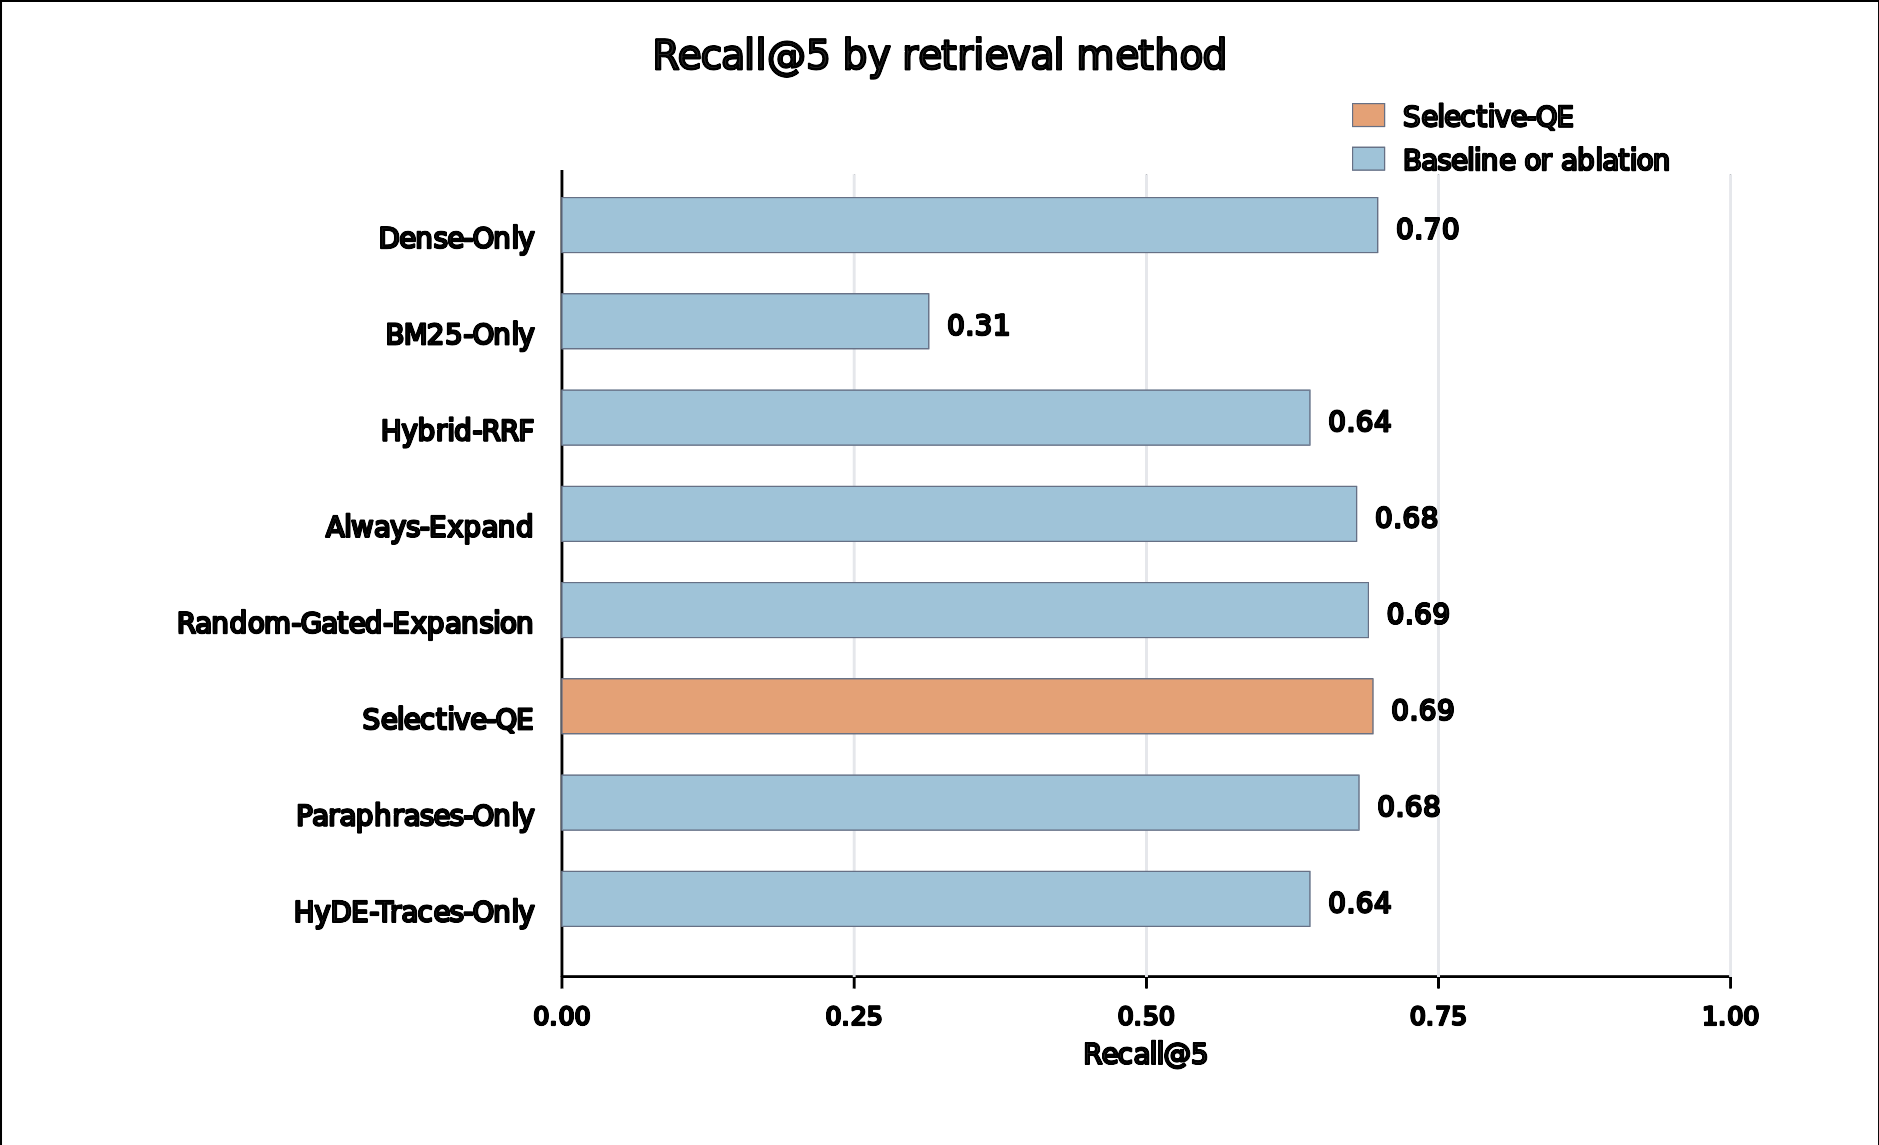
\includegraphics[width=0.95\linewidth]{figures/recall_at_5.png}
\caption{Recall@5 comparison across completed retrieval methods for seed 42. SQE is highlighted; the other bars are baselines or ablations.}
\Description{Bar chart comparing seed-42 Recall at 5 for dense retrieval, BM25, Hybrid-RRF, paraphrases, HyDE traces, always-expand, random-gated expansion, and SQE.}
\label{fig:recall}
\end{figure}

\section{Gate Diagnostics}
\begin{table}[!tbp]
\caption{Seed-42 gate diagnostic split by expansion decision.}
\label{tab:gate}
\centering
\small
\begin{tabular}{lrrrr}
\toprule
Subset & Count & Hits@5 & Misses@5 & Recall@5
\\
\midrule
Expanded & 230 & 142 & 88 & 61.7 \\
Not expanded & 270 & 205 & 65 & 75.9 \\
\bottomrule
\end{tabular}

\end{table}

Table~\ref{tab:gate} shows that the gate expands 230 of
500 queries. In the current run, expanded queries do not
outperform non-expanded queries at Recall@5, so top-1 dense score is not yet a
well-calibrated selector. This is a central weakness for the current method claim.
Stronger gates should include
top-1/top-2 margin, dense-sparse agreement, score concentration, or a learned
policy.

\subsection{Post-hoc threshold sweep}
\begin{table}[!tbp]
\caption{Seed-42 post-hoc threshold sweep.}
\label{tab:threshold-sweep}
\centering
\small
\begin{tabular}{rrrr}
\toprule
Threshold & Expanded & Recall@5 & Recall@10 \\
\midrule
0.45 & 0/500 & 69.8 & 75.4 \\
0.50 & 1/500 & 70.0 & 75.6 \\
0.55 & 17/500 & 70.0 & 75.6 \\
0.60 & 76/500 & 70.0 & 75.8 \\
0.62 & 130/500 & 70.2 & 76.2 \\
0.64 & 191/500 & 69.6 & 75.4 \\
0.65 & 230/500 & 69.4 & 75.4 \\
0.66 & 275/500 & 69.8 & 75.8 \\
0.68 & 340/500 & 69.0 & 75.8 \\
0.70 & 393/500 & 69.2 & 75.8 \\
0.75 & 478/500 & 68.0 & 75.6 \\
0.80 & 500/500 & 68.0 & 75.6 \\
\bottomrule
\end{tabular}

\end{table}

Table~\ref{tab:threshold-sweep} and Figure~\ref{fig:threshold} reuse the
completed dense-only and always-expand result files, so the sweep is
diagnostic rather than a tuned validation result. It indicates that the fixed
0.65 threshold is not optimal on this split, and threshold selection needs a
separate validation protocol.

\subsection{Split validation check}
\begin{table}[!tbp]
\caption{Seed-42 split validation check for threshold selection.}
\label{tab:validation-threshold}
\centering
\scriptsize
\begin{tabular}{lrrrr}
\toprule
Policy & Threshold & Expanded & Recall@5 & Recall@10 \\
\midrule
Dense-only proxy & 0.45 & 0/250 & 70.4 & 75.2 \\
Fixed gate & 0.65 & 115/250 & 71.2 & 77.6 \\
Validation-selected gate & 0.50 & 0/250 & 70.4 & 75.2 \\
\bottomrule
\end{tabular}

\end{table}

Table~\ref{tab:validation-threshold} reports a minimal guard against all-query
tuning: we select a threshold on the first half of the query IDs and report it on the second half. This split is small and
should not be treated as final evidence, but it makes the calibration weakness
explicit.

\subsection{Multi-seed gate validation}
\begin{table}[!tbp]
\caption{Held-out gate validation over independent memory-index seeds.}
\label{tab:multiseed-gate}
\centering
\scriptsize
\begin{tabular}{lrrrrr}
\toprule
Seed & Threshold & Train R@5 & Test R@5 & Dense Test R@5 & Expansion \\
\midrule
42 & 0.50 & 69.6 & 70.4 & 70.4 & 0.0 \\
43 & 0.60 & 70.0 & 64.0 & 63.6 & 17.2 \\
44 & 0.75 & 76.8 & 72.0 & 69.2 & 96.4 \\
45 & 0.75 & 71.2 & 73.6 & 69.6 & 97.6 \\
46 & 0.65 & 74.4 & 72.0 & 71.2 & 51.6 \\
47 & 0.45 & 65.6 & 68.4 & 68.4 & 0.0 \\
48 & 0.70 & 68.0 & 69.2 & 69.2 & 82.8 \\
49 & 0.60 & 68.4 & 64.4 & 63.6 & 19.6 \\
\midrule
Mean & -- & 70.5 & 69.2 & 68.2 & 45.6 \\
\bottomrule
\end{tabular}

\end{table}

Table~\ref{tab:multiseed-gate} repeats the split-threshold procedure for each completed
independent memory-index seed. It recombines only executed dense-only and
always-expand rows. The selected thresholds change mean test Recall@5 from 68.2\% for dense retrieval to 69.2\%, while expanding 45.6\% of held-out queries, but the result is still too
small to support a strong gate-calibration claim. A paired held-out test over 2000 query/seed pairs estimates a 1.1 point Recall@5 difference with a 95\% interval of [0.1, 2.1] and sign-flip $p=0.037$.
Table~\ref{tab:gate-paired} reports the paired test.

\begin{table}[!tbp]
\caption{Paired uncertainty for held-out gate validation.}
\label{tab:gate-paired}
\centering
\scriptsize
\begin{tabular}{lrrrrr}
\toprule
Scope & Queries & Gate R@5 & Dense R@5 & Delta & 95\% CI \\
\midrule
42 & 250 & 70.4 & 70.4 & +0.0 & [+0.0, +0.0] \\
43 & 250 & 64.0 & 63.6 & +0.4 & [-0.8, +2.0] \\
44 & 250 & 72.0 & 69.2 & +2.8 & [-1.2, +7.2] \\
45 & 250 & 73.6 & 69.6 & +4.0 & [+0.4, +7.6] \\
46 & 250 & 72.0 & 71.2 & +0.8 & [-2.0, +3.6] \\
47 & 250 & 68.4 & 68.4 & +0.0 & [+0.0, +0.0] \\
48 & 250 & 69.2 & 69.2 & +0.0 & [-4.0, +4.0] \\
49 & 250 & 64.4 & 63.6 & +0.8 & [-2.0, +3.6] \\
\midrule
All & 2000 & 69.2 & 68.2 & +1.1 & [+0.1, +2.1] \\
\bottomrule
\end{tabular}

\end{table}

\subsection{Cross-seed top-1 gate}
\begin{table}[!tbp]
\caption{Leave-one-seed-out top-1 gate validation.}
\label{tab:cross-seed-gate}
\centering
\scriptsize
\begin{tabular}{lrrrrrr}
\toprule
Test seed & Train seeds & Threshold & Gate R@5 & Dense R@5 & Delta & Expansion \\
\midrule
42 & 43,44,45,46,47,48,49 & 0.64 & 69.6 & 69.8 & -0.2 & 38.2 \\
43 & 42,44,45,46,47,48,49 & 0.62 & 66.6 & 66.4 & +0.2 & 27.6 \\
44 & 42,43,45,46,47,48,49 & 0.62 & 72.6 & 72.0 & +0.6 & 28.8 \\
45 & 42,43,44,46,47,48,49 & 0.62 & 69.8 & 69.0 & +0.8 & 28.8 \\
46 & 42,43,44,45,47,48,49 & 0.62 & 72.0 & 72.2 & -0.2 & 29.0 \\
47 & 42,43,44,45,46,48,49 & 0.64 & 67.4 & 67.0 & +0.4 & 42.6 \\
48 & 42,43,44,45,46,47,49 & 0.66 & 68.6 & 66.6 & +2.0 & 58.8 \\
49 & 42,43,44,45,46,47,48 & 0.64 & 66.4 & 65.0 & +1.4 & 41.2 \\
\midrule
All & -- & -- & 69.1 & 68.5 & +0.6 & 36.9 \\
\bottomrule
\end{tabular}

\end{table}

Table~\ref{tab:cross-seed-gate} selects a top-1-score threshold on two independent memory-index
seeds and evaluates it on the held-out seed. It recombines only executed
dense-only and always-expand rows. Leave-one-seed-out top-1 threshold selection obtains 69.1\% Recall@5 versus 68.5\% for dense retrieval while expanding 36.9\% of queries. The paired difference is 0.6 points with a 95\% interval of [-0.1, 1.3]. The interval
still crosses zero, so this result is useful as a calibration diagnostic rather
than a strong effectiveness claim.

\subsection{BM25-agreement gate variants}
\begin{table}[!tbp]
\caption{Held-out BM25-agreement gate variants.}
\label{tab:gate-variants}
\centering
\scriptsize
\begin{tabular}{llrrrr}
\toprule
Seed & Policy & Threshold & Test R@5 & Dense Test R@5 & Expansion \\
\midrule
42 & score\_and\_no\_bm25\_agreement & 0.50 & 70.4 & 70.4 & 0.0 \\
43 & score\_or\_no\_bm25\_agreement & 0.65 & 64.0 & 63.6 & 79.6 \\
44 & score\_only & 0.75 & 72.0 & 69.2 & 96.4 \\
45 & score\_or\_no\_bm25\_agreement & 0.70 & 73.6 & 69.6 & 90.4 \\
46 & score\_only & 0.65 & 72.0 & 71.2 & 51.6 \\
47 & score\_and\_no\_bm25\_agreement & 0.45 & 68.4 & 68.4 & 0.0 \\
48 & score\_and\_no\_bm25\_agreement & 0.70 & 68.8 & 69.2 & 55.6 \\
49 & score\_only & 0.60 & 64.4 & 63.6 & 19.6 \\
\midrule
Mean & -- & -- & 69.2 & 68.2 & 49.1 \\
\bottomrule
\end{tabular}

\end{table}

Table~\ref{tab:gate-variants} selects among score-only and BM25-agreement gate variants on
the first half of each seed and evaluates on the second half. It uses only
executed dense-only, BM25-only, and always-expand rows. The result is diagnostic:
the selected variants do not provide enough evidence to remove the gate
calibration limitation. Figure~\ref{fig:gate-diagnostic} shows why the
top-1 score is a weak selector in the current experiment.

\subsection{Gate headroom}
\begin{table}[!tbp]
\caption{Held-out oracle headroom for a perfect expansion gate.}
\label{tab:gate-headroom}
\centering
\scriptsize
\begin{tabular}{lrrrrr}
\toprule
Seed & Dense R@5 & Always R@5 & Oracle R@5 & Helpful & Harmful \\
\midrule
42 & 70.4 & 70.0 & 74.8 & 4.4 & 4.8 \\
43 & 63.6 & 63.6 & 68.0 & 4.4 & 4.4 \\
44 & 69.2 & 72.0 & 76.4 & 7.2 & 4.4 \\
45 & 69.6 & 73.6 & 76.0 & 6.4 & 2.4 \\
46 & 71.2 & 72.4 & 75.6 & 4.4 & 3.2 \\
47 & 68.4 & 68.0 & 73.6 & 5.2 & 5.6 \\
48 & 69.2 & 68.8 & 74.0 & 4.8 & 5.2 \\
49 & 63.6 & 66.0 & 69.2 & 5.6 & 3.2 \\
\midrule
Mean & 68.2 & 69.3 & 73.5 & 5.3 & 4.2 \\
\bottomrule
\end{tabular}

\end{table}

Table~\ref{tab:gate-headroom} recombines executed dense-only and always-expand rows
on the second half of each independent memory seed. The oracle column is not an
implementable method; it shows the maximum possible Recall@5 if a perfect gate
could expand exactly the queries helped by always-on expansion. The small gap
between helpful and harmful expansion cases explains why the current confidence
gate is difficult to calibrate.

\begin{figure}[!tbp]
\centering
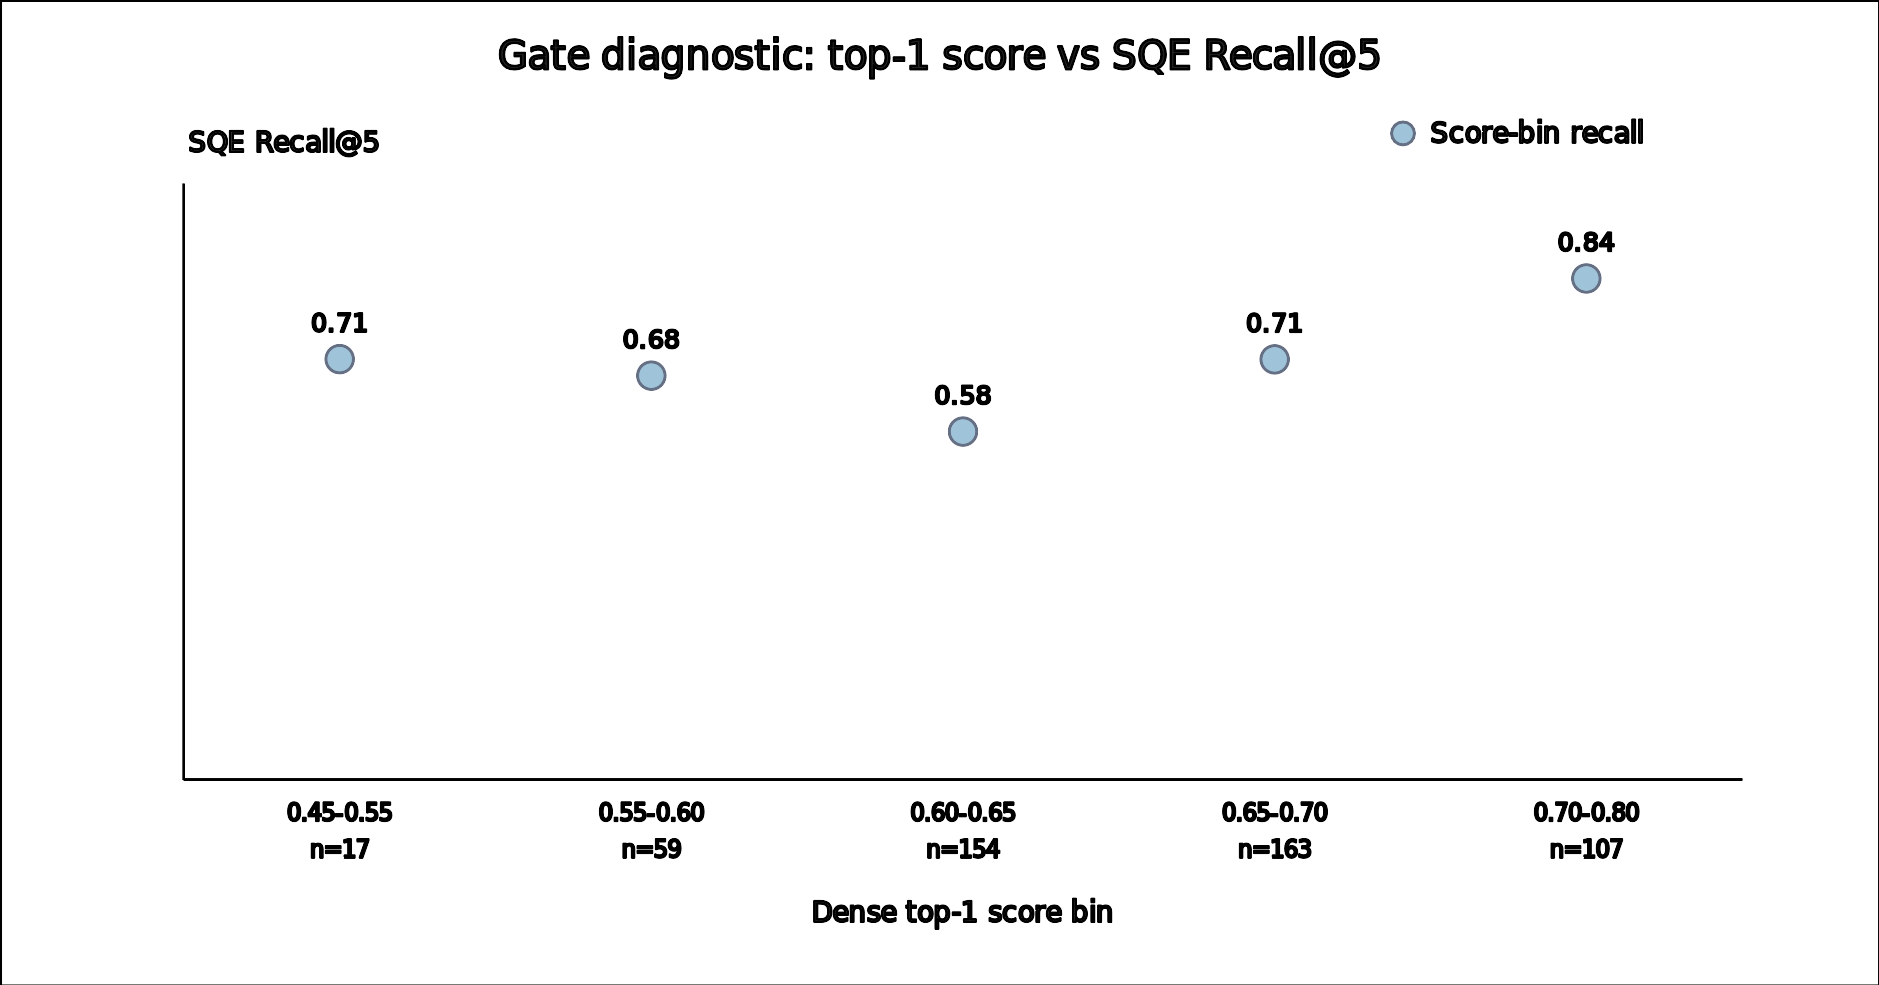
\includegraphics[width=0.95\linewidth]{figures/gate_diagnostic.png}
\caption{Diagnostic relationship between dense top-1 score bins and final SQE Recall@5. The bins do not separate easy and hard cases cleanly enough for a strong gate claim.}
\Description{Line and bar diagnostic showing that dense top-1 score bins do not provide a clean monotonic separation between higher and lower Recall at 5 outcomes.}
\label{fig:gate-diagnostic}
\end{figure}

\begin{figure}[!tbp]
\centering
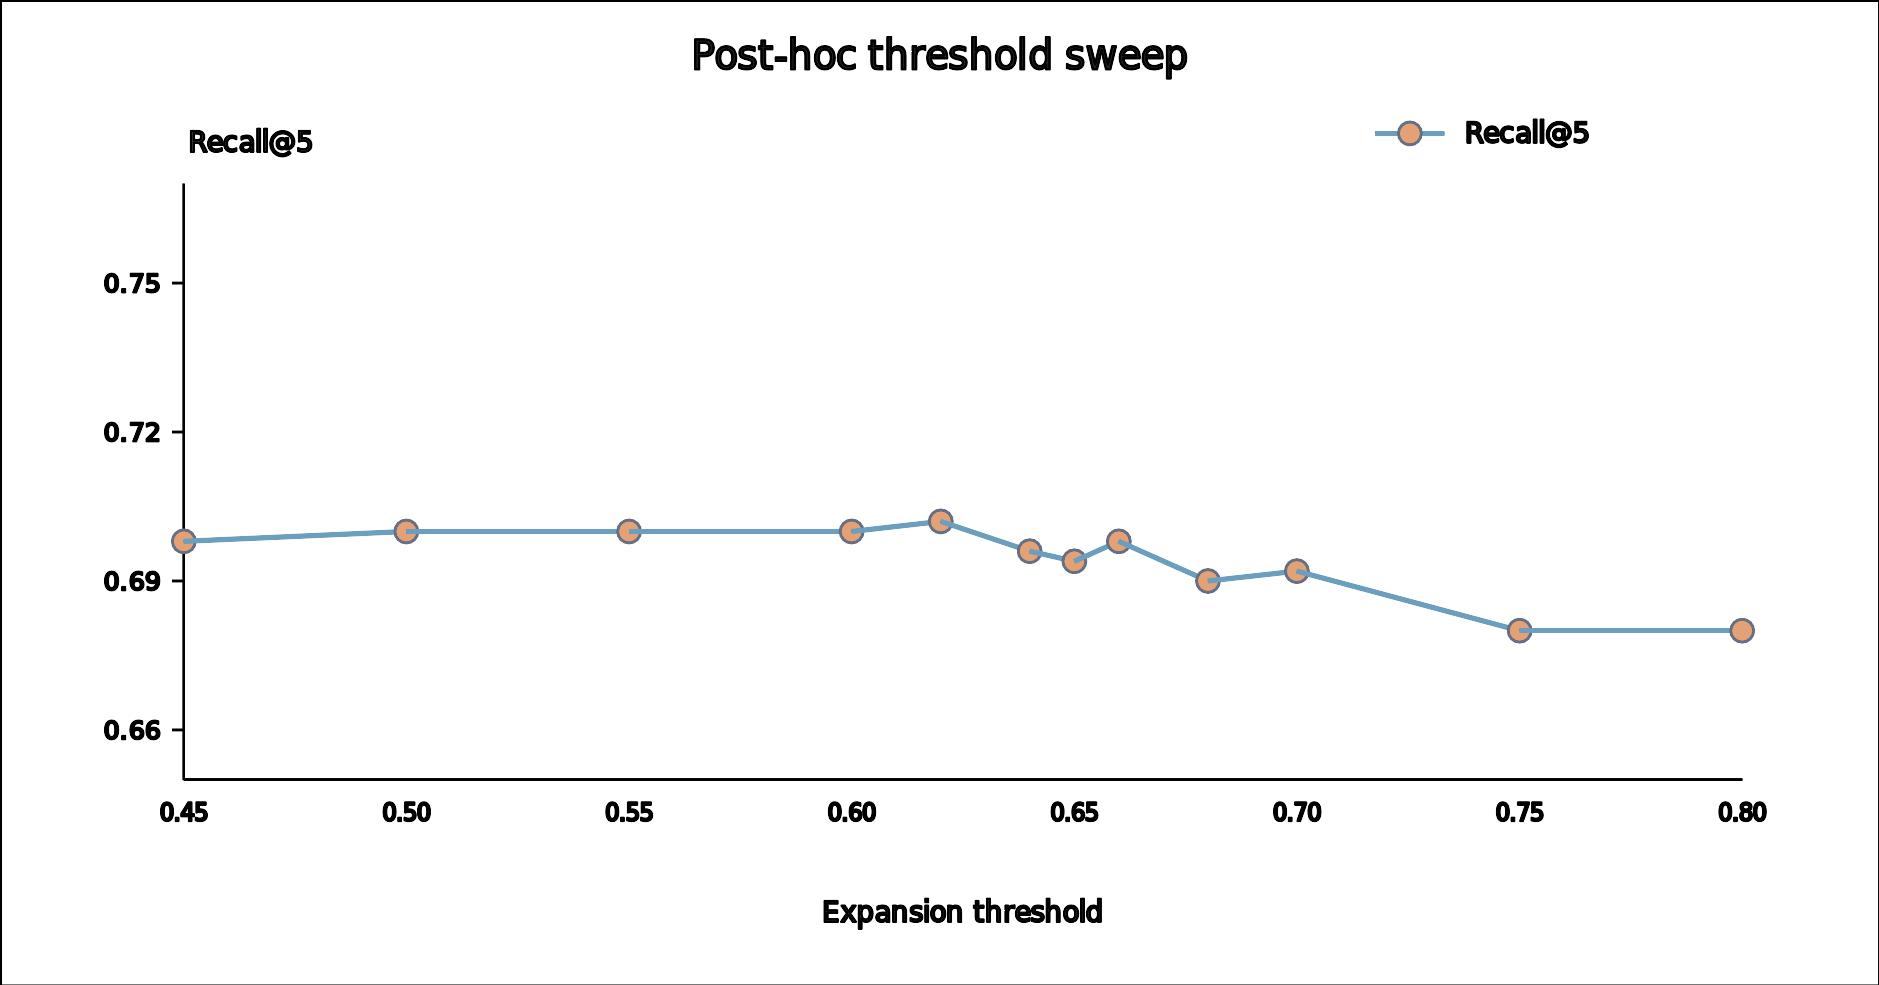
\includegraphics[width=0.95\linewidth]{figures/threshold_sensitivity.png}
\caption{Post-hoc Recall@5 under different expansion thresholds for seed 42. The figure is diagnostic because the threshold is evaluated on completed result rows.}
\Description{Threshold sweep chart showing post-hoc Recall at 5 as the expansion threshold changes for seed 42, with the fixed operating threshold marked for comparison.}
\label{fig:threshold}
\end{figure}

\section{Limitations and Next Experiments}
The current evidence is preliminary. The retrieval experiment now includes
8 independently rebuilt memory-index seeds, but the improvement over dense
retrieval is small and there is no downstream Pass@1 measurement. Simple
held-out gate diagnostics using top-1 score, dense margin, score concentration,
and BM25 agreement have not removed the calibration weakness. A stronger
submission needs externally validated gate calibration, human-audited query
labels, and end-to-end agent success measurements.

\section{Threats to Validity}
\paragraph{Construct validity.}
Recall@K measures whether the target memory appears in the retrieved set, not
whether an agent can use that memory to fix a software task. The current
retrieval metrics are therefore intermediate evidence. Pass@1 task success and
human query-quality labels are required before claiming agent-level gains.

\paragraph{Data validity.}
The evaluation queries are generated from the same memory corpus used to define
target memories. This gives a controlled retrieval benchmark, but it may not
match how users or agents phrase future memory requests. The human-audit packet
is prepared, but no reviewer labels have been collected yet.

\paragraph{Method validity.}
The selective gate uses top-1 dense score, which is weakly calibrated in the
current experiments. Several held-out diagnostics test alternative gates, but
their intervals still cross zero. The current results should be read as a
cost-controlled retrieval study rather than evidence that the gate is solved.

\paragraph{External validity.}
The experiments use SWE-smith software-engineering traces, BAAI/bge-m3
embeddings, and Qwen3.6-35B-A3B for expansion. Results may change with other
agent logs, embedding models, generators, memory-writing policies, or task
domains.

\section{Reproducibility}
The intended public repository URL is: \texttt{TODO: add GitHub URL}.
The intended Hugging Face dataset URL is:
\texttt{TODO: add Hugging Face dataset URL}.
All scripts used for the current retrieval experiment are in the project
directory. Raw seed-42 results are stored under \nolinkurl{results_500_memory_seed42/},
and generated paper artifacts are stored under \texttt{paper/}. Independent
memory-index seed results are stored under the
\nolinkurl{results_500_memory_seed42/} through
\nolinkurl{results_500_memory_seed49/} directories.
The verifier \nolinkurl{scripts/07_verify_experiment.py} checks that evaluation
targets are present in both the memory store and the index, recomputes retrieval
metrics from detailed JSONL files, and verifies required paper artifacts.
The dataset-release helper \nolinkurl{scripts/33_prepare_hf_dataset_release.py}
packages existing memory stores, evaluation pairs, retrieval summaries,
diagnostics, and the unlabeled human-audit packet into a local Hugging
Face-ready directory. It does not create human labels, downstream Pass@1 rows,
or synthetic replacement data.
The code-release helper \nolinkurl{scripts/34_prepare_github_code_release.py}
prepares a local GitHub-ready code package with scripts, paper source, configs,
documentation, and optional lightweight summaries. It does not upload to
GitHub and does not package raw memory stores, detailed query rows, downstream
task-outcome rows, or human labels.
The table inventory \nolinkurl{paper/table_inventory.json} records the source
files for each active table; deprecated diagnostic tables are excluded from the
paper claims.

\section{Conclusion}
SQE is a retrieval-time query-expansion method for long-horizon software-agent
memory. In the current experiments, it reduces expansion calls relative to
always-on expansion and improves Recall@5 over Hybrid-RRF and trace-only
expansion, but it remains essentially tied with dense retrieval and the executed
random-gating budget control. The present evidence is best read as a
verified retrieval study and a negative calibration result for the
current top-1-score gate. A stronger paper requires human-audited query labels
and downstream Pass@1 task-success measurements before making agent-level
performance claims.

\bibliographystyle{plain}
\bibliography{references}
\end{document}
